\documentclass[11pt]{article}
\usepackage{amssymb,amsmath,amsthm}
\usepackage{bm, mathrsfs}
\usepackage{graphicx}
\usepackage{geometry}
\usepackage{textcomp}
\usepackage{hyperref}
\usepackage{ragged2e}
\usepackage{float}
\graphicspath{ {./images/} }
\newtheorem{remark}{Remarque}
\newcommand{\bx}{\bm{x}}

\title{ISC3, Fall 2022 (A22) \\
 Computer works report TP 2, 26/09/2022}
\author{Wenlong CHEN}
\date{October 6 2022}

\begin{document}
    \maketitle
    \section{Stem}
    From a dataset point cloud, we want to achieve a regression using the following regression function defined on [0, 1]:
        \begin{equation}
        \Tilde{f}_d(x) = \sum\limits_{j=1}^{d}u_j\Lambda_j(x) \qquad where \qquad \Lambda_j(x)=\max\left(0,1-(d-1)\left|x-\frac{j-1}{d-1}\right|\right)
    \end{equation}
    This function defines a piecewise linear function. Try and analyze the following Scilab script:
    \begin{verbatim}
    clear
    function y = piecewiselinear(x,d,u)
    y = zeros(x);
    for j = 1:d
    y = y + u(j)*max( 0, 1-(d-1)*abs(x-(j-1)/(d-1)) );
    end
    endfunction
    //
    //Example
    d=10;
    xi = linspace(0,1,d);
    u = sin(2*%pi*xi);
    x = linspace(0,1,200);
    y = piecewiselinear(x, d, u);
    plot(x, y, ’-’); plot(xi, u, ’o’); xgrid();
    \end{verbatim}
    Consider the following dataset generated by the following Scilab script
    \begin{verbatim}
    N=100;
    xi = rand(N,1);
    yi = sin(2*%pi*xi)+0.2*rand(N,1, "normal");
    \end{verbatim}
    Then we want to find the coefficients uj , j = 1, ..., d, that minimize the least square error
        \begin{equation}
        \min\limits_{\left( u_1,\ldots,u_d \right)} {\frac{1}{2}\sum\limits_{j=1}^{N} \left( \Tilde{f}_d(x_i)-y_i \right)^2}
    \end{equation}
    (the coefficients $u_j$ are in the definition of $\title{f}$).


    \section{Questions}

    a) On the paper, determine what is $A_{ij}$ . Then in a Scilab script, assemble the matrix
    $A \in \emph{M}_{Nd}(R)$.\\
    Solution :\\
    $$A_{ij}=\Lambda_j(x_i)=\max\left(0,1-(d-1)\left|x_i-\frac{j-1}{d-1}\right|\right)$$
    ~\\

    \raggedright
    b) Solve the normal equations $A^T Au = A^T y$. \\
    Code pour cette question :
    \begin{verbatim}
        function y = piecewiselinear(x,d,u)
            y = zeros(x);
            for j = 1:d
                y = y + u(j)*max( 0, 1-(d-1)*abs(x-(j-1)/(d-1)) );
            end
        endfunction

        N=100;d=20
        xi = rand(N,1);xi = gsort(xi);
        yi = sin(2*%pi*xi)+0.2*rand(N,1, "normal");

        A = zeros(N,d)
        for j=1:d
            A(:,j) = max( 0, 1-(d-1)*abs(xi-(j-1)/(d-1)) );
        end

        coefs = (A'*A)\(A'*yi)
    \end{verbatim}
    ~\\

    c) By using the function piecewiselinear(), plot the resulting regression function in
    solid line. On the same graphics, plot also the point cloud $\left(x_i,y_i\right)_{i=1,\ldots,N}$ with circles for each point. Check if the resulting function $\title{f}(x)$is a good regression function.\\
    Solution : 
    \begin{figure}[H]
        \centering
        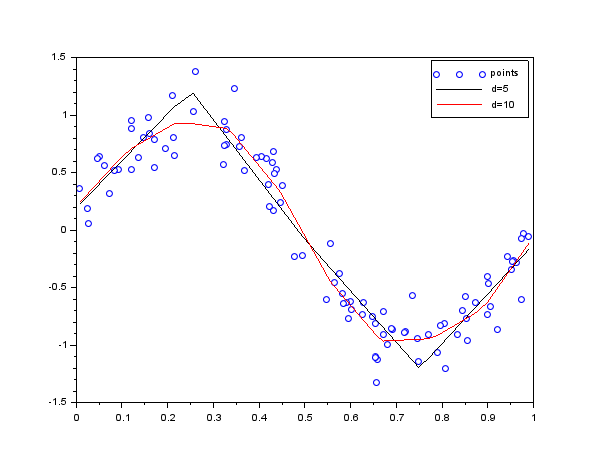
\includegraphics[width=0.8\textwidth,height=0.5\textwidth]{piece}
        \caption{L'image de la function piecewiselinear}
    \end{figure}

    ~\\
    Next, we would like to add a Tykhonov regularization term to the least square
    minimization problem, and study the effect of the regularization coefficient $\mu<0$.\\
    ~\\

    d) Consider a set of regularization coefficients $\mu_k = 10^k, k = -8,\ldots,2$.\\
    For each k solve the regularized normal equations
    \begin{equation}
        \left(A^TA+\mu_kI\right)u_k=A^Ty
    \end{equation}
    (u now depends on k, so we add an index k in $u_k$ to notice the dependency). Then
    plot the regression function $\title{f}_d(x)$ and the point cloud on the same graphics as before.
    Observe the (possible) influence of the regularization coefficient $\mu_k$ on the solution.\\
    Solution : 
    \begin{figure}[H]
        \centering
        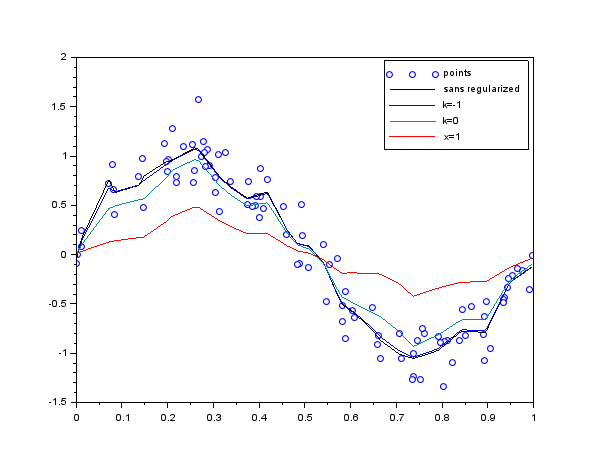
\includegraphics[width=0.8\textwidth,height=0.5\textwidth]{regu}
        \caption{la function piecewiselinear ave la regularization}
    \end{figure}

    Code pour cette question :
    \begin{verbatim}
        coefs2=zeros(d,10)
        for k=1:10
            uk=10^(k-9)
            coefs2(:,k) = (A'*A+uk.*eye(d,d))\(A'*yi)
        end
        plot2d(xi,piecewiselinear(xi,d,coefs2(:,8)),style=2)
        plot2d(xi,piecewiselinear(xi,d,coefs2(:,9)),style=16)
        plot2d(xi,piecewiselinear(xi,d,coefs2(:,10)),style=5)
        legend("points","sans regularized", "k=-1","k=0","x=1");
    \end{verbatim}
    ~\\

    e) On another graphics, plot the parametric curve
    \begin{equation}
    \mu_k\rightarrow\left(\left||Au_k-y\right||,\left||u_k\right||\right)^T
    \end{equation}
    still for $\mu_k = 10^k, k = -8, \ldots, 2$, and plot the parametric curve in log-log scale. Inyour opinion, what could be the best empirical value of $\mu_k$ ?
    \begin{figure}[H]
        \centering
        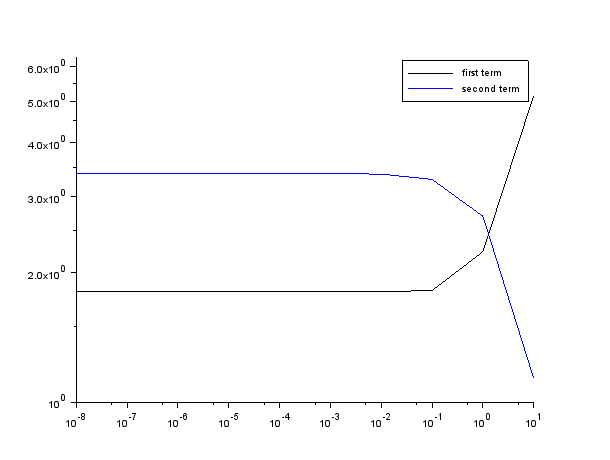
\includegraphics[width=0.8\textwidth,height=0.5\textwidth]{imag}
        \caption{the parametric curve}
    \end{figure} 
    Nous choisissons le point d'intersection des deux lignes, qui est proche de $x=0$, lorsque $k=0,u_k=0$

    \section*{Résumé}
    Une dimensionnalité élevée crée des problèmes d'ajustement excessif, qui peuvent être résolus en réduisant la dimensionnalité ou en ajoutant une régularisation afin d'atténuer l'ajustement excessif.
 \end{document}